\chapter{Davis' Construction}\label{c3}

This\pageoriginale lecture is devoted to sketching the proof of Theorem
\ref{c2:thm2.5}.

\begin{step}\label{c3:step1}
  We can assume that $K$ is a compact smooth manifold with
  boun\-dary. For example, embed $K$ in $\mathbb{R}^n$ for some
  $n$. Then replace $K$ with a regular neighbourhood of it.
\end{step}

\begin{step}\label{c3:step2}
  Let $K$ be a smooth manifold with boundary and $T$ be a piecewise
  smooth triangulation of $\partial K$. Let $V$ and $E$ denote the set
  of vertices and edges of $T$, respectively. Associate to $T$ the
  group $\Gamma$ generated by the vertices $v \in V$ with the
  relations $v^2 =1$ if $v \in V$ and $(uv)^2=1$ if $\{ u, v\} \in
  E$. For each subset $S$ of $V$, $\Gamma (S)$ denotes the subgroup of
  $\Gamma$ generated by $S$. We identify a simplex $\sigma$ of $T$
  with the subset of $T$ consisting of the vertices of $\sigma$;
  consequently, $\Gamma (\sigma)$ is defined. For $v \in V$, let
  $D(v)=$Star $(v)$ be the closed dual cell of $v$ in the first
  barycentric subdivision of $T$. For each simplex $\sigma$ in $T$,
  its dual cell 
  $$
  D(\sigma) = \prod \{ D(v)\}
  $$
  where $v$ varies over the vertices of $\sigma$. The dual cells give
  a regular cell complex structure to $\partial K$. To each $x \in
  \partial K$ associate the subgroup $\Gamma_x =\Gamma(\sigma)$ of
  $\Gamma$, where $\sigma$ is the unique simplex such that $x \in $
  Interior $D (\sigma)$. If $x \in$ Interior $K$, then define
  $\Gamma_x=\{1\}$. Define $\mathcal{M}= K \times T/ \sim$, where $(x,
  \alpha) \sim (y, \beta)$ if and only if $x=y$ and $\alpha^{-1} \beta
  \in \Gamma_x$. There is an abvious action of $\Gamma$ on $\mathcal{M}$;
  i.e., $g[x, h]= [x, gh]$ for $g \in \Gamma$ and $[x, h]\in
  \mathcal{M}$. (Compare J. Tits \cite{95}.) Note that the orbit space
  $\mathcal{M}/\Gamma =K$. 
\end{step}

\begin{step}\label{c3:step3}
  This step is devoted to proving the following result.
\end{step}

\begin{lemma}\label{c3:lem3.1}
  Provided $T$ is a first barycebtric subdivision of a simplicial
  complex $F$, then $\Gamma(S)$ is a finite (Coxeter) group if and
  only if $S$ is a simplex of $T$.
\end{lemma}

\begin{proof}
  If $S$ is a simplex of $T$, then all the elements in $\Gamma(S)$
  commute and hence are of order two. Therefore,
  $\Gamma(S)=(\mathbb{Z}/2)^{|S|}$. Concersely, if $\Gamma (S)$ is
  finite, then for each pair $v \neq w$ in $S$ we must have $\{ v, w\}
  \in E$; otherwise, $\Gamma (S)$ would map onto an infinte dihedral
  group. We will now use the assumption that $T$ is a first
  barycentric subdividion of\pageoriginale a simplicial complex $F$; i.e., the
  vertices $V$ of $T$ are the simplices of $F$. Note that $V$ is
  partially ordered by the face relation on the simplices of $K$. The
  simplices of $T$ are the totally ordered subsets of $V$; i.e., the
  subsets for which every pair of elements are comparable. But we have
  just seen that if $v \neq w \in S$, then $\{ v, w\}$ is a simplex of
  $T$; hence $v$ and $w$ are comparable. This implies that $S$ is a
  simplex of $T$.
\end{proof}

\begin{example*}
  Let $K$ be a 2-simplex  and $T$ be the 1-skeleton of $K$, then
  $\Gamma$ is the finite group $\mathbb{Z}_2 \oplus \mathbb{Z}_2 \oplus
  \mathbb{Z}_2$. But this does not contradict Lemma \ref{c3:lem3.1}
  since $T$ is not the first barycentric subdivision of anything. Note
  in this example that $\mathcal{M}$ is the octahedron.
\end{example*}

\begin{figure}[H]
\centering{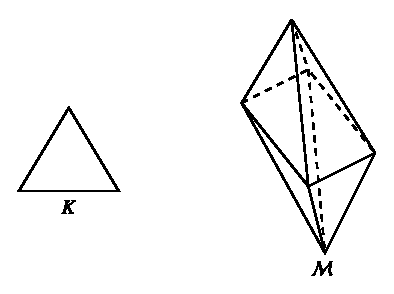
\includegraphics{vol86-figures/fig2.eps}}\\
Figure 2
\end{figure}

\begin{step}\label{c3:step4}
  We may assume during the remainder of the proof of Theorem
  \ref{c2:thm2.5} that $T$ is the first barycentric subdivision of
  some simplicial complex $K$; e.g., replace $T$ by its first
  barycentric subdivision. Hence, Lemma \ref{c3:lem3.1} is applicable
  to $T$. Since $\Gamma$ is a Coxeter group, it has a faithful
  representation into $GL_{|V|}(\mathbb{R})$. Consequently, by a
  result of Selberg \cite{87}, $\Gamma$ contains a normal subgroup
  $\prod$ of finite index such that $\prod$ is torsion free. In this
  case, $\prod$ can be taken to the kernel of the obvious epimorphism
  $\Gamma \to \mathbb{Z}_2^{|V|}$ where $\mathbb{Z}_2^{|V|}$ is the
  abelianization of $\Gamma$. Using the fact (from Lemma
  \ref{c3:lem3.1}) that $\Gamma _x$ is a finite Coxeter group for each
  $x \in K$, Davis shows that $\mathcal{M}= \mathcal{M} / \prod$ is a
  closed manifold. Let $G= \Gamma/\prod$, then $G$ acts on $M$ and
  $M/G= \mathcal{M}/\Gamma=K$. Now the maps $K \to M \to M/G=K$
  demonstrate that\pageoriginale $K$ is a retract of $M$.
\end{step}

\begin{step}\label{c3:step5}
  Using the fact (from Lemma \ref{c3:lem3.1}) that $\Gamma (S)$ finite
  implies $S$ is a simplex of $T$, Davis shows that the group elements
  in $\Gamma$ can be enumerated as $g_1, g_2, \ldots $ so that the
  following statement $(*)$ holds:
  \begin{equation*}
    \mathcal{M}_n \cap (K \times g_{n+1}) ~\text{is contractible,
      where }~ \mathcal{M} = \cup \left\{K \times g_i | 1 \leq i \leq
    n \right\}. \tag{$*$}
  \end{equation*}
\end{step}

The intersection in $(*)$ is, in fact, homeomorphic to
$\mathbb{D}^{m-1}$ where $m = \dim K$. Consequently, if $K$ is
contractible, so is each $\mathcal{M}_n$; and if $K$ is aspherical, so
is each $\mathcal{M}_n$. It follows that $\mathcal{M}$ is contractible
when $K$ is contractible. Likewise, $K$ aspherical implies
$\mathcal{M}$ is aspherical which in turn implies $M$ is
aspherical. This completes our sketch of the proof of Theorem
\ref{c2:thm2.5}. 

\begin{remark}\label{c3:rem1}
  We see by $(*)$ that $\mathcal{M}_n$ is a manifold with
  boundary. Also, $\partial M_{n+1}= \partial \mathcal{M}_n \#
  \partial K$; therefore
  $$
  \pi_1 (\partial \mathcal{M}_n) = \pi_1 (\partial K)* \ldots * \pi_1
  (\partial K), n ~\text{factors},
  $$
  provided $\dim K > 3$. Here $*$ denotes free product. This means
  that $\mathcal{M}$ is not simply connected at infinity if $\pi_1
  (\partial K)\neq \{ 1\}$. In particular, $\mathcal{M}$ is not
  homeomorphic to $\mathbb{R}^m$. Now it is well known that there
  exist $K$, for each $m \geq 4$, such that $K$ is contractible but
  $\partial K$ is not simply connected. In this way, Davis \cite{21}
  gets his example of a closed aspherical manifold whose universal
  cover is not $\mathbb{R}^m$.
\end{remark}

\begin{remark}\label{c3:rem2}
  The example due to Davis and Hausmann \cite{23} of a closed
  aspherical manifold which does not support a smooth structure is
  constructed by first finding a compact, piecewise linear, aspherical
  manifold $K$ with non-empty boundary such that the interior of $K$
  does not support a smooth structure. (Davis' construction does not
  need that $K$ is smooth; it only uses the triangulation $T$ of
  $\partial K$.) Well known results from smoothing theory yields such
  a $K$. Consequently, $M = \mathcal{M}/\prod$ does not support a
  smooth structure. If it did, then so would $\mathcal{M}$ and any
  open subset of $\mathcal{M}$; in particular, the interior of $K$.
\end{remark}

\begin{remark}\label{c3:rem3}
  The example of Davis and Januskiewicz \cite{24} require new ideas
  employing Gromov's hyperbolization construction \cite{54}.
\end{remark}
